\section{Configuration Problem }\label{sec: Problem Definition}

The configuration problem is characterised by \textit{components} which have  \textit{properties}. 
The domains of these components are given by a set of \textit{component types}.
Additionally, the domain of the component properties is given by the predefined property values of the corresponding component types.
There are configuration constraints that put restrictions on the presence of components, and the values of their properties.   
The task is to create a configuration solution, which is an assignment of types to components, along with values to their properties that satisfy the constraints. \newline 

To illustrate the problem, it is applied to the configuration of a bike. 
The task is to create a bike that satisfies all the user requirements, along with other constraints.
Just like a configuration, a bike has different components of which it is composed (compare Figure \ref{fig:bike}).
Components of this bike are the bike (as the root component), frame, front wheel, rear wheel, basket, and stand. 
Component types for the frame are for example f1, f2, or f3 which represent bike frames available in the inventory. 
The property values of the component types are already given, for example, the size of wheel w1 is 28.
The domain property of a component, for example, the size of the front\_wheel, can be 26 or 28 and be made of aluminum or carbon fiber depending on the component type w1, w2, or w3. 
When choosing aluminum wheels with the size 28, w1 has to be part of the configuration. 
A list with all components and their attributes and possible attribute values can be found in the appendix. 


\begin{landscape}
\begin{figure}[]
\centering
\caption{Bike Configuration in UML}
    \label{fig:bike}
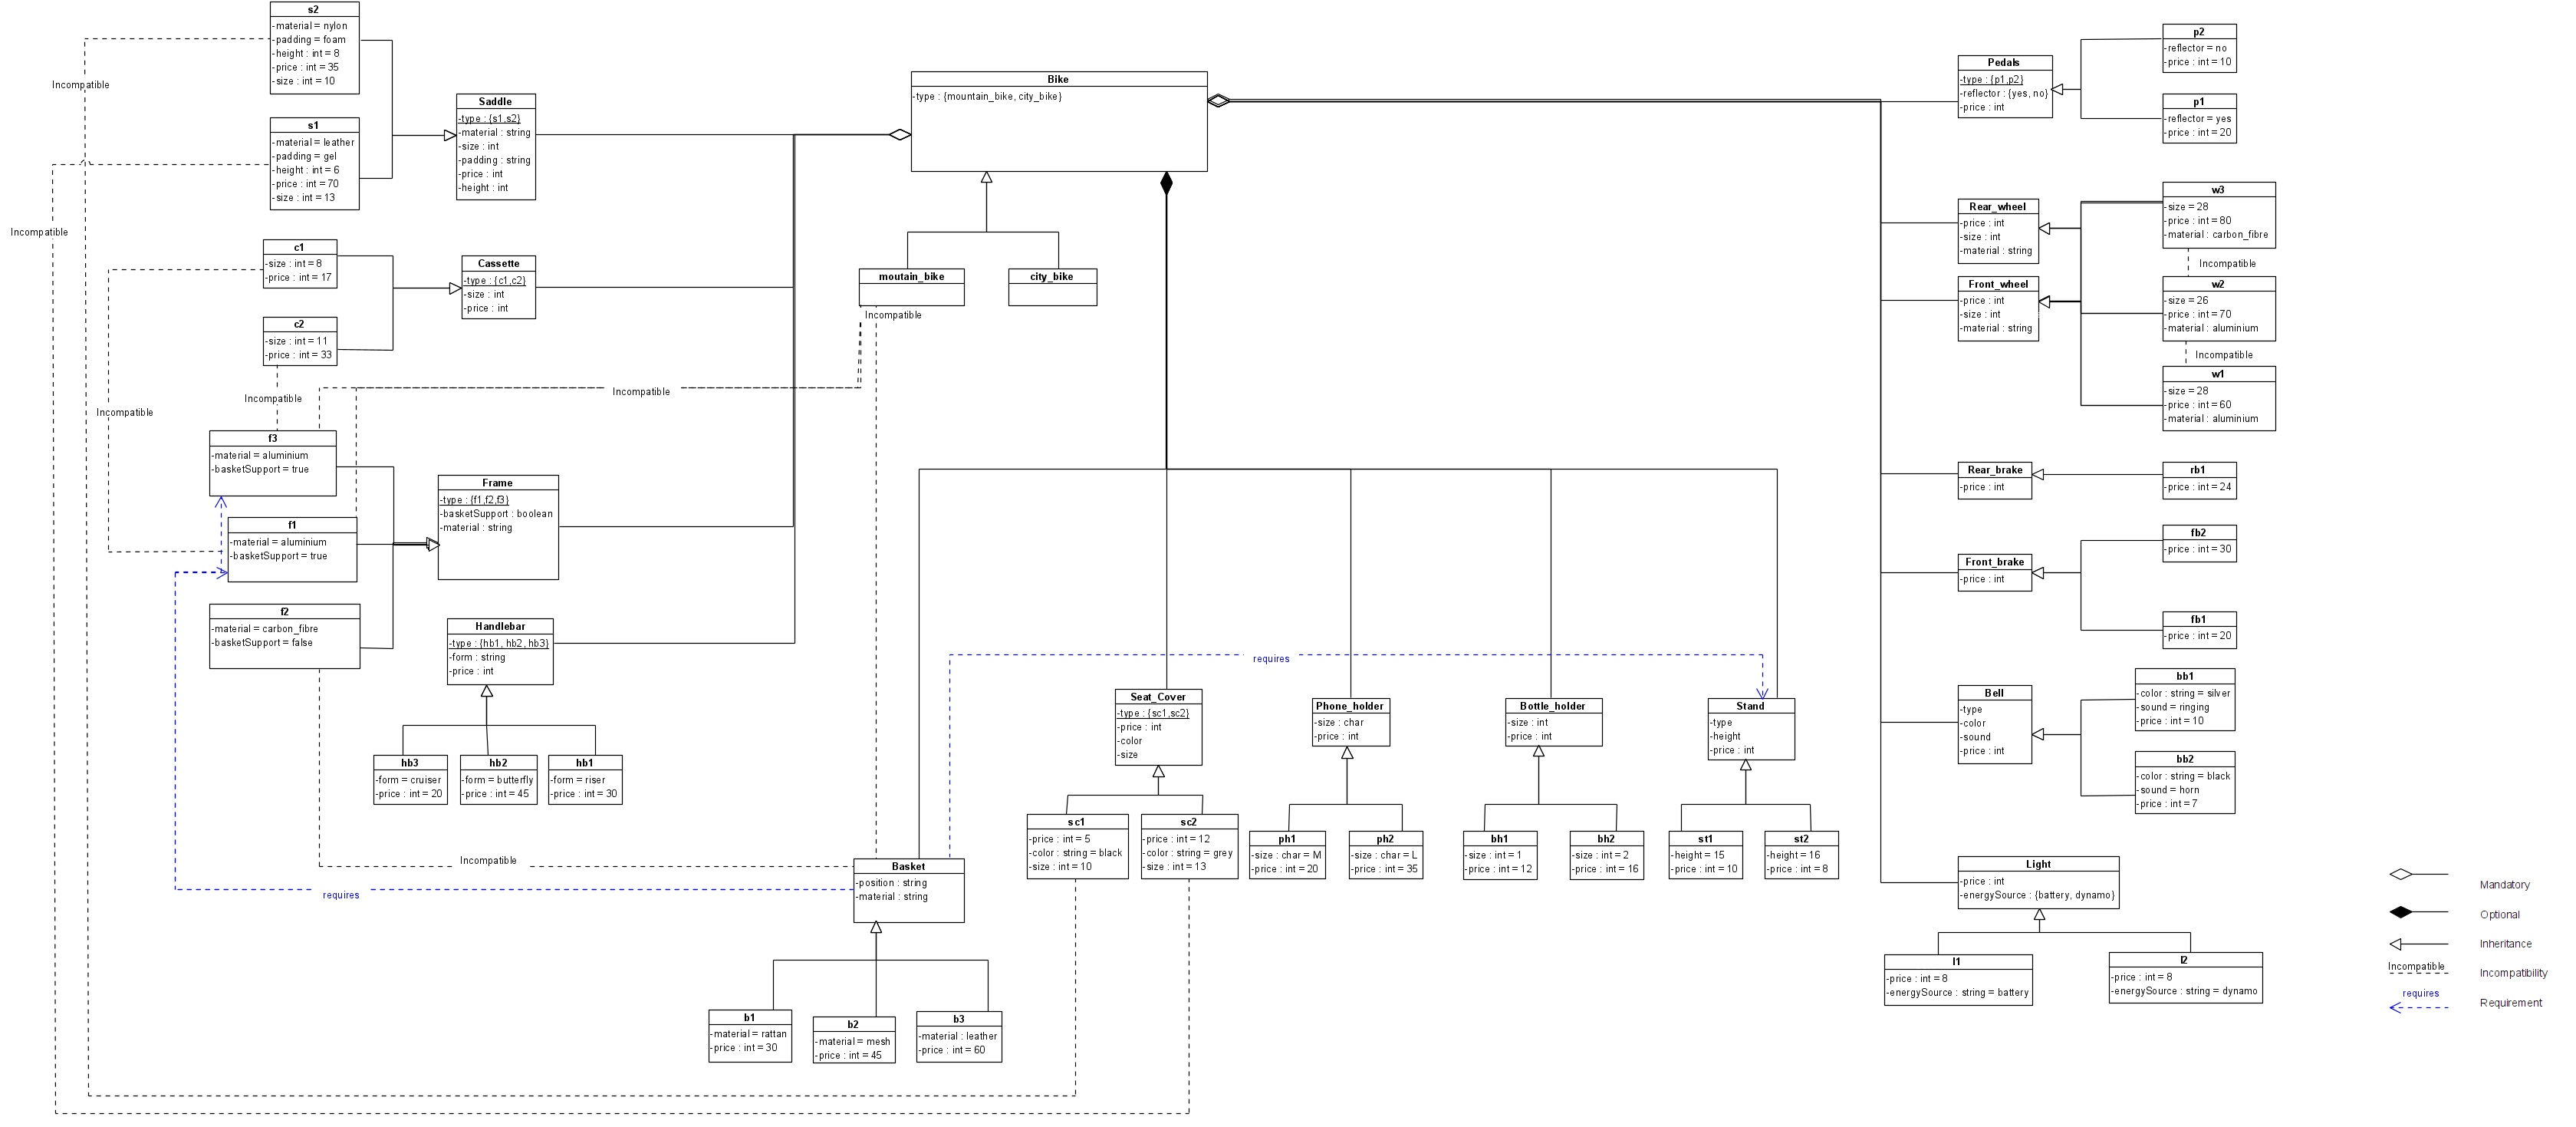
\includegraphics[height=0.6\textheight,width=1.5\textwidth,keepaspectratio]{Bike.jpg}
\end{figure}

\end{landscape}

\subsection{Configuration Constraints}
To fully describe the configuration problem, we need the configuration knowledge base (components, properties, and their domains) along with the constraints.
In the background section, I have already analysed various constraints that must be satisfied for a successful configuration: inheritance-relationships, whole-part-relations, incompatibility, compatibility, resource, require, and user requirements. 
In addition, certain properties can be mandatory or be set to default values. 
The configuration constraints that are considered in this thesis are listed below. \newline

\noindent \textbf{Property value Assignment}: Property of components must be assigned values from their domains as per their component type. For the assignment of values to component properties, 4 constraints must be fulfilled. 
\begin{itemize}
 \item \textbf{A1}: Every component present in the configuration solution must be assigned a component type.
 \item \textbf{A2}: A component property can only have one value. 
 \item \textbf{A3}: The values assigned to a component property must exactly correspond to the predefined property values of the component type it is assigned.
 \item \textbf{A4}: All mandatory properties of a component should be assigned values if the component is in a configuration solution.
\end{itemize}

\noindent \textbf{Partonomy}: The partonomy (whole-part-relations) reveals the structure of a product. A component can have part components. All components can either be optional or mandatory. For example, a bike frame and the wheels are mandatory components whereas the stand is an optional component. 
\begin{itemize}
\item \textbf{P1}: If a part component is present in an assignment, the whole component must be also in the configuration. 
\item \textbf{P2}: If a component is present in an assignment, all the mandatory part components have to be in the assignment. 
\end{itemize}

\noindent \textbf{Requirements}: Requirement constraint ensures that in order for a component (with property values) to be present in the solution, other components (with property values) are also needed in the solution. There can be three different cases of requirements for a configuration.
\begin{itemize}
\item \textbf{R1}: A component requires another component to be part of the solution.
\item \textbf{R2}: To satisfy the configuration, a component requires another component with a specific property value to be assigned to the configuration (or vice versa). 
\item \textbf{R3}: To satisfy the configuration, a component with a certain property value requires another component with a specific property value to be assigned to the configuration. 
\end{itemize}

\noindent \textbf{Incompatibility}: Incompatibility prevents certain component types and their property values from appearing together in a configuration. 
For this problem, two components with specific property values can be incompatible. 
The case that a combination of several components is incompatible with a single (or a set of) components is not covered. 
\begin{itemize}
\item \textbf{I1}: Incompatible components cannot be together in a configured solution. 
\item \textbf{I2}: A component can be incompatible with a certain presence value of another component. In this case, if the former component is present in the solution, then the later component can't have the respective property value. 
\item \textbf{I3}: The property value of a component can be incompatible with the property value of another component. In this case, only one of the components and their property value can be part of the solution or both have to be excluded. 
\end{itemize}

\noindent \textbf{User Requirements}: A customer or user can specify special requirements for the configuration in terms of components, component types, or property values. 
\begin{itemize}
\item \textbf{U1}: Every component that the user requests, must be part of the configuration.
\item \textbf{U2}: A user can require a component with a specific property value. In this case, the specified component with the respective property value must be present in the solution. 
\item \textbf{U3}: Every component that the user requests not to be present, must not be part of the configuration.
\item \textbf{U4}: A user can require that a component with a specific property value is not in the configuration. In this case, the specified component may be absent or may be present with another value for the respective property in the solution. 
\end{itemize}

In the literature, it is suggested to treat incompatibility and compatibility as replacements of each other \cite{hofestrybawo14a}. Meaning, only one concept should be used depending on whether the majority of the components are either compatible or incompatible. 
Compatibility constraints could be stated in the same way as \textbf{I1},  \textbf{I2} and \textbf{I3}, and the difference would be that if a component with or without some property value is present, then only the compatible component with or without component values have to be present.
For the bike problem, most components are compatible with each other and only a few are incompatible.
A basket, for example, is incompatible with a mountain bike. 
Therefore, the incompatibility rules I1-I3 are included in the encoding. \newline

For future work, \textit{resource constraint} (including pricing constraints) or \textit{default values} can be included as configuration constraints. The resource constraints are usually domain-specific, and the aim of this work is to clearly separate the domain or product knowledge from the configuration knowledge for the encoding. Therefore, they are not covered by this encoding. However, those constraints have to fulfill certain requirements. \newline

\subsection{Cases}
For a better understanding of the configuration problem, I will introduce three use cases with different user requirements. The first user needs a city bike, the second a mountain bike, and the third user does not specify which bike they prefer but chooses components with a low price (if specified). The user requirements are listed in the tables below. \newline

For the bike problem, the mandatory components are divided into two different categories. First are the components needed for a bike to work like a frame, pedals, cassette, saddle, rear wheel, front wheel, and handlebar. The second category consists of components required by German law like front and rear light, brakes, and a bike bell \cite{stvzo}. The presence of those components in a configuration is non-negotiable.

\subsubsection{Requirements User 1: City Bike}

The first user requires a city bike and has specified the requirements for nearly all components.  Only the requirements for the basket are not specified.  Also, the user doesn't want a bottle holder or a seat cover. 

\begin{table}[]
\centering
\begin{tabular}{llll}
\hline
Component     & Required   (Y/N) & Specification           & Component type \\ \hline 
Bike          & Y                & bike = city bike        & City bike      \\
Basket        & Y                & -                       & any            \\
Cassette      & Y                & size = 8                & c1             \\
Rear wheel    & Y                & size = 26               & w2             \\
Front wheel   & Y                & size = 26               & w2             \\
Frame         & Y                & material = Carbon fibre & f3             \\
Handlebar     & Y                & form = Butterfly        & hb2            \\
Light         & Y                & energy source = Battery & l1             \\
Pedals        & Y                & clip pedals = true      & p1             \\
Front brake   & Y                & price = 20              & fb1            \\
Rear brake    & Y                & price = 24              & rb1            \\
Saddle        & Y                & padding = Gel           & s1             \\
Bike bell     & Y                & colour = silver         & bb1            \\
Phone holder  & Y                & price = 20              & ph1            \\
Bottle holder & N                &                         &                \\
Seat cover    & N                &                         &                \\
Stand         & Y                & height = 16             & st2            \\ \hline \end{tabular}
\caption{Requirements User 1}
\label{tab:userreq1}
\end{table}                                   

\subsubsection{Requirements User 2: Mountain Bike}
For the mountain bike, the second user does not require a phone holder or a bike stand. The details of the frame are not specified, because there is only one frame that is compatible with the mountain bike.
Also, a basket is not compatible with it. 

\begin{table}[H]
\centering
\begin{tabular}{llll}
\hline
Component       & Required   (Y/N)  & Specification             & Component type   \\ \hline
Bike            & Y                 & bike = mountain bike      & Mountain bike \\
Cassette        & Y                 & size = 11                 & c2              \\
Rear wheel      & Y                 & material= carbon fibre    & w3              \\
Front wheel     & Y                 & material= carbon fibre    & w3              \\
Handlebar       & Y                 & form = riser              & hb1             \\
Light           & Y                 & energy source = Dynamo    & l2              \\
Pedals          & Y                 & clip pedals = false       & p2              \\
Front brake     & Y                 & price = 30                & fb2             \\
Rear brake      & Y                 & price = 24                & rb1             \\
Saddle          & Y                 & material = Nylon          & s2              \\
Bike bell       & Y                 & colour = black            & bb2             \\
Phone holder    & N                 &                           &               \\
Bottle   holder & Y                 & price = 12                & bh1             \\
Seat cover      & Y                 & -                         & any             \\ 
Stand           & N                 &                           &          \\      \hline
\end{tabular}
\caption{Requirements User 2}
\label{tab:userreq2}
\end{table}

\subsubsection{Requirements User 3: Price Sensitivity}
The third user is price sensitive. This person always prefers the less expensive option. Only the frame component and the bike type have no price attribute. Therefore, all three frame types and the two bike types are possible. The user doesn't need any optional components to reduce the price of the bike. 

\begin{table}[H]
\centering
\begin{tabular}{llll}
\hline
Component       & Required   (Y/N) & Specification          & Component type \\ \hline
Bike            & Y                & -                      & any  \\
Cassette        & Y                & price = 17             & c1            \\
Rear wheel      & Y                & price = 60             & w1            \\
Front wheel     & Y                & price = 60             & w1            \\
Handlebar       & Y                & price = 20             & hb3           \\
Light           & Y                & price = 8              & l1            \\
Pedals          & Y                & price = 20             & p1            \\
Front brake     & Y                & price = 20             & fb1           \\
Rear brake      & Y                & price = 24             & rb1           \\
Saddle          & Y                & price = 35             & s2            \\
Bike bell       & Y                & price = 7              & bb2           \\
Phone holder    & N                &                        &               \\
Bottle   holder & N                &                        &               \\
Seat cover      & N                &                        &               \\
Stand           & N                &                        &               \\ \hline
\end{tabular}
\caption{Requirements User 3}
\label{tab:userreq3}
\end{table}